\documentclass[a4paper]{article}

\usepackage{tecnico_relatorio}


\usepackage[hypcap]{caption} % makes \ref point to top of figures and tables
\usepackage{rotating}
\usepackage{multirow}

\begin{document}
	\trSetImage{img/tecnico_logo}{6cm} % Logotipo do Técnico
	\trSetSubject{Arquitecturas Avançadas de Computadores}
	\trSetType{Laboratório III - Paralelização e Aceleração de um Programa}

	
	\trSetBoxStyle{0.3}
	
	\trSetAuthorNr{3}
	
	\trSetAuthors
	{
		\begin{center}
			Gonçalo Ribeiro

			73294
		\end{center}
	}{
		\begin{center}
			Miguel Costa

			73359
		\end{center}
	}{
		\begin{center}
			Rafael Gonçalves

			73786
		\end{center}
	}
		
	\trSetProfessor{Prof. Leonel Sousa}
	
	\trMakeCover
	
	\tableofcontents
	\pagebreak
	
	\section{Introdução}
	
	O objectivo do presente trabalho laboratorial é a aceleração e paraleliazação de um algoritmo de \textit{smoothing}. Foi dada a possibilidade de realizar este projecto recorrendo a instruções vectoriais ou utilizando um processador gráfico, sendo que se escolheu utilizar instruções vectoriais suportadas pela arquitectura Intel IA32e (MMX, SSEx, AVX). 
	
	O algoritmo de \textit{smoothing} consiste na obtenção de uma função aproximada, em que é filtrado todo o rído resultante da amostragem do sinal. Na \autoref{fig:fun_smoothing} estão representados dois gráficos, em que o primeiro demostra o sinal com ruído e o segundo a função resultante após se aplicar \textit{smoothing}.
	
		\begin{figure}[h]
			\centering
			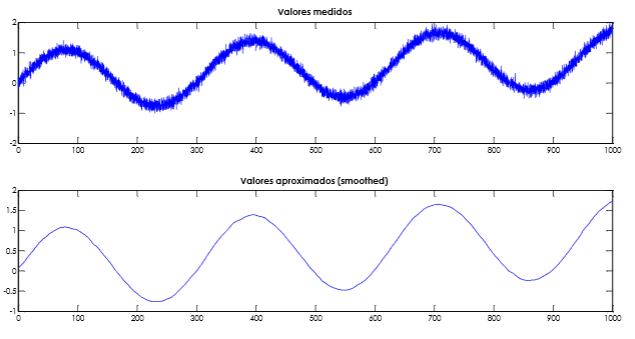
\includegraphics[width=1.\textwidth]{img/fun_smoothing}
			\caption{Resultado da aplicação de \textit{smoothing} a um sinal com ruído. }
			\label{fig:fun_smoothing}
		\end{figure}
		
	Para calcular o \textit{smoothing} foi fornecida a equação que permite calcular o valor aproximado $\hat{y}$$ _1$, $...$ , $\hat{y}$$ _{N-1}$, tendo em conta a função observada no domínio $x$$ _1$, $...$ , $x$$ _{N-1}$, dando origem aos pontos $y$$ _1$, $...$ , $y$$ _{N-1}$:
	
	\begin{equation}
		\hat{y}_i =  \frac{ \sum_{k=0}^{N-1} K_b (x_i, x_k ) y_k}{\sum_{k=0}^{N-1} K_b (x_i, x_k )} 
		\label{eq:smoothing_function}
	\end{equation}
	
	Onde
	
	\begin{equation}
		K_b (x_i,x_k)=exp\left(-\frac{(x-x_k)^2}{2b^2} \right)
		\label{eq:smoothing_kb}
	\end{equation}
	 	
	 	 
	Também é já fornecido um algoritmo (algoritmo 1) que ilustra um exemplo para calcular o resultado da função de \textit{smoothing}.
	
	
	\section{Aceleração e Paralelização}
	
	Para realizar a aceleração do programa foram adoptadas várias estratégias: usando instruções de processamento vectorial de 128 bits e usando instruções de processamento vectorial de 128 bits com \textit{unrolling} do ciclo de computação em 2, 3, 4 e 8 cálculos por ciclo.
	
	A primeira tarefa a executar é então alocar o espaço necessário para a computação. Para tal usou-se uma função já forncida pelo professor ($aligned\_malloc$) que permite alocar um tamanho desejado de memória, incluindo algum espaço adicional. De seguida são corridos os algoritmos em teste, ou seja, é corrido o algoritmo 1, seguido dos vários algoritmos de aceleração de modo a se poder obter um termo comparativo entre cada estratégia adoptada e o algoritmo original. 
	
	Note-se que antes de se medir qualquer tempo, o algoritmo em análise é corrido, de modo a poder-se preencher à partida algumas posições da cache. Isto é feito não só para os algoritmos de aceleração, como também para o algoritmo 1 de modo a haver consistência nos resultados.
	
	Após se obterem os diversos valores temporais, é liberta a memória anteriormente alocada e são verificados os resultados de \textit{smoothing} obtidos de modo a comprovar se se chegou na verdade ao desejado: remover o ruído de um sinal.
	
	\subsection{\textit{Smoothing} Simples}
	
	Para realizar a operação de \textit{smoothing} foi usada a expressão anteriormente mencionada mas usando operações vectoriais, ou seja, para realizar a soma, subtração, multiplicação e divisão foi usado, respectivamente, as funções $\_mm\_add\_ps$, $\_mm\_sub\_ps$, $\_mm\_mul\_ps$ e $\_mm\_div\_ps$. Além destas funções foram usadas outras funções que permitem fazer \textit{load} ou \textit{store} de certos dados.
	
	\subsection{\textit{Smoothing} com \textit{Unroll} nos ciclos de computação}
	
	Para tentar acelerar ainda mais o algoritmo desenvolvido, foi testado a execução de \textit{unrolling} no ciclo de computação. Nesse sentido foram testados 4 casos de \textit{unrolling}: 2, 3, 4 e 8 instruções por ciclo, sendo que se pode concluir que o aumento de instruções por ciclo tende a aumentar ligeiramente o speedup obtido.
	
	
	\section{Testes} 
		
	Para testar a aceleração do nosso programa foram comparados os tempos de execução do algoritmo 1 com os programas desenvolvidos pelo grupo para acelerar o algoritmo 1. A tabela seguinta demonstra o tempo de execução do algoritmo 1 (Tempo Original) e os \textit{speedups} encontrados para diferentes tamanhos de vectores (entre 16 e 16384 \textit{floats}) para as várias estratégias desenvolvidas:
	
	\begin{table}[h]
		\centering
		\begin{tabular}{lllllll}
\multirow{2}{*}{Tamanho do Vector} & \multirow{2}{*}{Tempo Original {[}{]}} & \multicolumn{5}{l}{SSE-128 Speedup}                                                              \\
                                   &                                        & \textit{Simples} & \textit{Unroll 2} & \textit{Unroll 2} & \textit{Unroll 2} & \textit{Unroll 2} \\
16                                 & 4.6                                    & 0.884615         & 0.958333          & 0.410714          & 0.920000          & 0.171642          \\
32                                 & 61.2                                   & 3.090909         & 3.600000          & 4.935484          & 5.563636          & 4.309859          \\
64                                 & 237.4                                  & 2.799528         & 3.618902          & 2.580435          & 3.450581          & 3.440580          \\
128                                & 929.4                                  & 3.812141         & 10.707373         & 10.146288         & 4.732179          & 4.302778          \\
256                                & 2006.2                                 & 4.965842         & 5.876391          & 5.591416          & 6.393244          & 5.499452          \\
512                                & 4689.4                                 & 3.082698         & 3.663021          & 3.795241          & 3.982167          & 3.940010          \\
1024                               & 21119.0                                & 2.736969         & 3.145236          & 3.231478          & 3.362470          & 3.361292          \\
2048                               & 93695.2                                & 2.919054         & 3.363386          & 3.491712          & 3.595585          & 3.606880          \\
4096                               & 408000.6                               & 3.171430         & 3.693677          & 3.836525          & 3.947367          & 3.982164          \\
8192                               & 1634784.8                              & 3.165204         & 3.724790          & 3.882026          & 3.964539          & 4.029549          \\
16384                              & 6482300.2                              & 3.153480         & 3.879947          & 3.882026          & 3.960604          & 4.029549          \\
32768                              & 25781057.0                             & 3.144238         & 3.711833          & 3.877029          & 3.953504          &                   \\
                                   &                                        &                  &                   &                   &                   &                   \\
                                   &                                        &                  &                   &                   &                   &                  
\end{tabular}
\end{table}
	
	\section{Demonstração \textit{vs.} Desenvolvido}
	
	 Aquando a demonstração, os resultados de speedup obtidos eram muito inferiores ao esperado (estando-se a obter valores de speedup próximos de 1). Contudo, após uma análise mais detalhada sobre o funcionamento de instruções vectoriais, verificou-se que, apesar da não se estar a usar a porção de código correspondente ao uso de instruções de processamento vectorial para 256 bits, o facto de existir esta porção de código fazia com que o compilador agendasse mudanças de modo entre o processamento de 128 bits e o de 256 bits, o que atrasava imenso a execução do programa. Como tal separam-se estas duas componentes de processamento em dois programas distintos. Esta simples mudança fez com que, ao usar as instruções de processamento de 128 bits, se conseguisse atingir resultados de speedup próximos do esperado.
	   
	
	
	
	\section{Conclusão}

\end{document}
